\section{Blokų grandinės technologija}

Blokų grandinė - tai vieno su kitu susijusių blokų grandinė, kurios blokuose saugomi
nekeičiami įrašai \cite{SatoshiNakamoto}. Šią technologiją galima apibūdinti kaip daugybę paskirstytų nekintamų skaitmeninių įrašų 
(angl. \textit{immutable distributed ledger}), tarpusavyje susietų taikant kriptografiją (blokų grandinės pavyzdys pateikiamas~\ref{fig:blockchain} paveiksle). Technologija geriausiai žinoma dėl jos panaudojimo Bitcoin kriptovaliutoje.
Šiame skyriuje apžvelgiami pagrindiniai blokų grandinės techniniai aspektai, savybės bei galimi skirtingi variantai.

\begin{figure}[H]
    \centering
    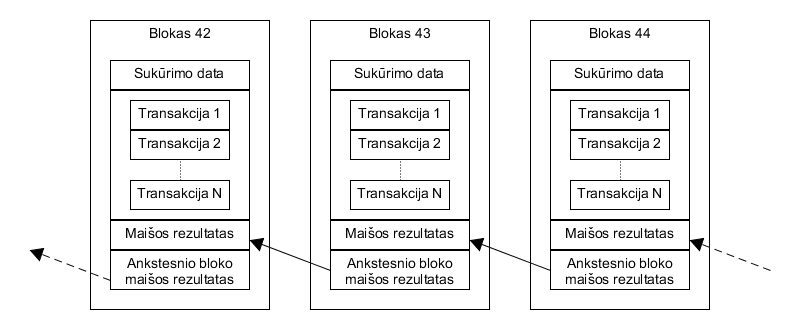
\includegraphics[scale=0.6]{img/blockchain}
    \caption{Supaprastintas blokų grandinės modelis}
    \label{fig:blockchain}
\end{figure}

\subsection{Nekintamumas}

Blokų grandinėje kiekvienas blokas yra sudarytas iš šių dalių:

\begin{enumerate}
    \item transakcijų. Kiekviena transakcija yra duomenys, kuriuos norima saugoti blokų grandinėje. Šie duomenys gali būti bet kokia vertinga informacija:
    finansinės transakcijos, programinis kodas, asmens duoti sutikimai (angl. \textit{consents}) ar kt. Kiekviena transakcija yra pasirašoma
    kūrėjo privačiu raktu. Vienas blokas gali turėti vieną arba daugiau transakcijų;
    \item bloko kriptografinės maišos funkcijos rezultato (angl. \textit{hash});
    \item ankstesnio (tėvinio) bloko kriptografinės maišos funkcijos rezultato;
    \item bloko sukūrimo laiko. Blokai grandinėje saugomi chronologiškai;
    \item kitų metaduomenų (pvz. bloko eilės numerio, blokų grandinės versijos, \textit{nonce} darbo įrodymui).
\end{enumerate}

Kiekvieno bloko maišos funkcijos rezultatas priklauso nuo jo transakcijų, prieš tai buvusio bloko maišos rezultato ir bloko metaduomenų.
Jeigu betkurio bloko duomenys būtų pakeisti, tuomet maišos funkcija sugeneruotų kitokį maišos rezultatą ir būtų lengva patikrinti, kad
naujai perskaičiuotas maišos rezultatas nesutampa su bloke esančiu rezultatu. Taip pat, kadangi kiekvienas blokas
priklauso nuo prieš tai buvusio bloko, net ir pakeitus vieną iš pirmųjų blokų, pakeitimas būtų pastebimas pridedant naujus blokus ir būtų galima suprasti,
kad turima blokų grandinės versija yra nevalidi (žr.~\ref{fig:blockchainNotIntact} pav.). Tokiu būdu kiekvienas blokų grandinės blokas patvirtina prieš tai
buvusio bloko integralumą, taip pasiekiant blokų grandinės nekintamumą (angl. \textit{immutability}),
nes perrašyti įrašus blokuose nepastebėtam labai sunku \cite{SatoshiNakamoto}.

\begin{figure}[H]
    \centering
    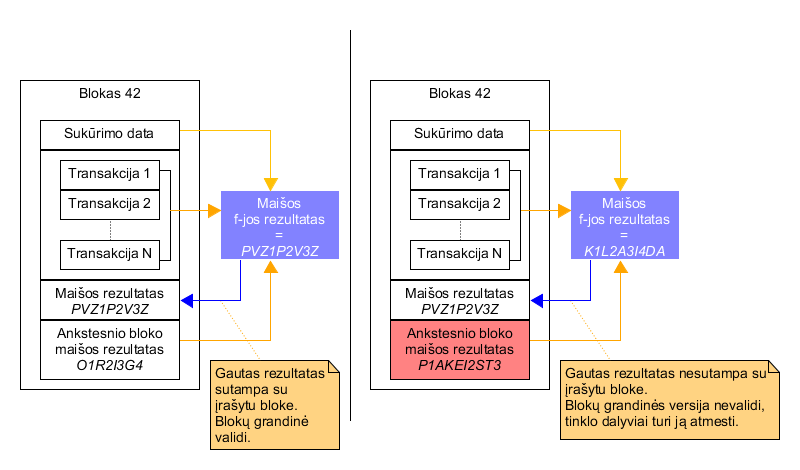
\includegraphics[scale=0.6]{img/blokchainNotIntact}
    \caption{Bloko grandinėje validavimas}
    \label{fig:blockchainNotIntact}
\end{figure}

\subsection{Decentralizuotumas}

Blokų grandinės sistema yra decentralizuota. Sistemą sudaro daugybė blokų grandinės mazgų (angl. \textit{node}), kurie turi visą blokų grandinės kopiją. Šie mazgai
yra atsakingi už naujų transakcijų validavimą, blokų su transakcijomis kūrimą, sukurtų blokų priėmimą į blokų grandinę ir pranešimus kitiems mazgams apie naują į grandinę priimtą
bloką \cite{Antonopoulos2016}.

Kadangi nėra centrinės institucijos, kuri nuspręstų, ar siūlomas blokas yra tinkamas priimti į grandinę, sprendimą bendrai turi priimti
visi tinklo dalyviai. Egzistuoja skirtingos taisyklės, vadinamos konsensuso strategijomis (plačiau apie juos~\ref{blockchain:consensus} skyrelyje), kuriomis
remdamiesi tinklo mazgai nusprendžia, ar pasiūlytas blokas yra validus. Šios taisyklės apibrėžia, kaip tinklo dalyviai turi įrodyti bloko validumą jį siūlydami į grandinę
bei kaip patikrinti kito dalyvio pasiūlyto bloko validumą.

\subsection{Konsensuso strategijos} \label{blockchain:consensus}

Kadangi blokų grandinės sistema yra decentralizuota, nėra centrinės institucijos, kuri nuspręstų, ar naujai siūlomas pridėti į grandinę blokas
yra validus (be transakcijų su falsifikuotais duomenimis). Taip pat, tinklo grandinės dalyviai neturėtų aklai pasitikėti kitais tinklo dalyviais - 
viešoje blokų grandinėje jie gali būti programišiai. Todėl blokų grandinės tinkle taikoma konsensuso strategija,
pagal kurią nusprendžiama, ar pridėti naują bloką į grandinę. Pateikiamos trys dažniausiai naudojami konsensuso strategijos.

\subsection{Darbo įrodymo (angl. \textit{proof of work})}

Darbo įrodymo konsensuso strategija remiasi principu, kad daug pastangų ir resursų į bloko validumo įrodymą įdėjęs tinklo
dalyvis nebus linkęs sukčiauti. Šioje strategijoje tinklo dalyvis, norėdamas pridėti bloką į blokų grandinę, turi išspręsti laikui ir resursams
imlų matematinį
uždavinį (užsiima \textit{bloko kasimu}). Pirmas uždavinio reikšmę radęs tinklo dalyvis praneša apie ją kitiems, kurie turi patvirtinti,
ar ši reikšmė teisinga. Jei tai patvirtinta, tinklo dalyviai patikrina, ar naujojo bloko transakcijos yra validžios. Jeigu jos validžios,
blokas pridedamas į grandinę \cite{Zheng2017}.\\
Darbo įrodymo matematinis uždavinys būna paremtas kriptografine maišos funkcija, kurios rezultatą lengvą validuoti,
tačiau duomenis, sugeneravusius šį rezultatą, sunku surasti. Uždavinio tikslas ir būna surasti šiuos duomenis. Tinklo dalyviai eikvoja didžiulius kiekius energijos ir laiko,
nes radimas būna paremtas duomenų perrinkimu (angl. \textit{brute force}). Dėl šios priežasties rezultato ieškantiems tinklo dalyviams
(vadinamiems \textit{kasėjais}) neretai būna įvestas paskatinimo sistema, kuri teisingą reikšmę radusį
\textit{kasėją} apdovanoja piniginiu atlygiu \cite{SatoshiNakamoto}. 

Kadangi blokų grandinės tinklas yra decentralizuotas, įmanoma situacija, kad labai panašiu metu į grandinę skirtingų mazgų pridėti du validūs blokai.
Taip dalis tinklo dalyvių gaus vieną mazgą, o dalis - kitą, o abu jie bus susieti su tuo pačiu prieš tai buvusiu bloku.
Tokiu atveju, taikoma ilgiausios grandinės taisyklė (žr.~\ref{fig:blockchainLongestRule} pav.). Mazgai dirba prie pirmiau gauto bloko,
tačiau išsaugo kitą gautą bloką kaip šaką. Po to, kai bus gautas dar vienas blokas, jis bus susietas tik su viena iš šakų - taip ši šaka taps ilgesnė. Tuomet
ilgesnė šaka paskelbiama aktyviąja grandine, visi su trumpesniąja šaka dirbę mazgai turi pereiti prie aktyviosios grandinės, o atmesto bloko (vadinamo \textit{bloku-našlaičiu}) transakcijos
grąžinamos į bendrą transakcijų sankaupą (angl. \textit{transaction pool}) \cite{SatoshiNakamoto}.
Realiuose blokų grandinės taikymuose, dažnai laukiama keleto iš eilės einančių naujų blokų, kad būtų galima atmesti \textit{bloką-našlaitį}. Pavyzdžiui,
Bitcoin blokų grandinėje laukiama apytiksliai 6 blokų, kad \textit{bloką-našlaitį} būtų galima atmesti \cite{Zheng2017}.


\begin{figure}[H]
    \centering
    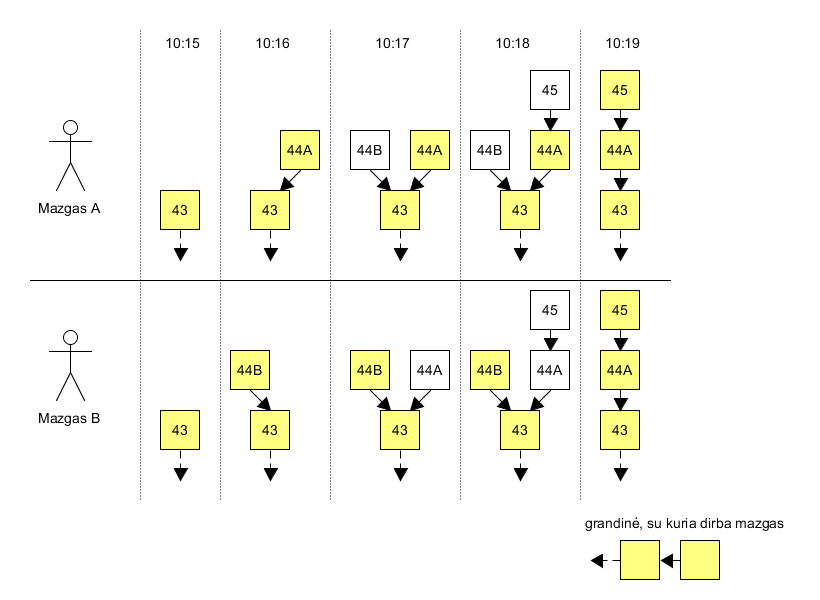
\includegraphics[scale=0.6]{img/blockchainLongestRule}
    \caption{Ilgiausios grandinės taisyklės taikymas}
    \label{fig:blockchainLongestRule}
\end{figure}

\subsubsection{Turto įrodymo (angl. \textit{proof of stake})}

Turto įrodymo konsensuso strategija remiasi principu, kad daug blokų grandinės turto turintis kasėjas
bus sąžiningas, nes išaiškinus jo nesąžiningumą jis rizikuoja prarasti savo turimą turtą \cite{Baars2016}. Šis algoritmas patiki sprendimą priimti
tiems tinklo dalyviams, kurie įrodo kad turi daugiausia turto (pvz. blokų grandinės kriptovaliutos). Tai gali pasirodyti kaip nesąžiningas sprendimas,
nes turtingiausias tinklo dalyvis gali būti vienvaldžiu sprendimų priėmėju. Dėl to blokų grandinės tinklai neretai taiko šios strategijos
variantus: Peercoin papildomai vertina turto amžių, Blackcoin kitą patvirtintoją paskiria pagal atsitiktinę funkciją, kuri atsižvelgia ir į turimą turtą \cite{Zheng2017}.

Ši strategija leidžia nebeeikvoti didžiulių elektros kiekių, skirtingai nei darbo įrodymo strategijoje \cite{Ethereum}. Algoritmo efektyvumas
taip pat sutaupo laiko ir blokai būna greičiau patvirtinami ir pridedami į grandinę. Tačiau, dėl praktiškai nulinių bloko \textit{kasimo} sąnaudų,
galimos dažnesnės tinklo atakos \cite{Zheng2017}. 

\subsubsection{Įtakos įrodymo (angl. \textit{proof of authority})}

\subsection{Viešumo tipai}

